\documentclass[12pt]{book}
\usepackage[margin=2cm, bindingoffset=0cm]{geometry}
%\usepackage[german]{babel} 
\usepackage[ngerman]{babel} %sudo apt-get install texlive-lang-german
\usepackage{hyperref} % web links etc.
\usepackage[parfill]{parskip}
\usepackage[utf8]{inputenc}
\usepackage[dvipsnames]{xcolor}
\usepackage{tcolorbox}
\usepackage{helvet} 
\usepackage{framed}
\usepackage{anyfontsize}
\usepackage{csquotes}
\MakeOuterQuote{"}
\definecolor{quotecolor}{rgb}{0.8,0.9,1}
\renewcommand{\familydefault}{\sfdefault} 
\setlength\parindent{0pt}
\tcbset{width=0.9\textwidth,boxrule=0pt,colback=quotecolor,arc=0pt,auto outer arc,left=0pt,right=0pt,boxsep=5pt}

\begin{document}
\title{\fontsize{40}{40}\selectfont \textbf{Die Schrift}}
\date{\today}
\maketitle

\chapter{Wozu diese Schrift?}

Diese Schrift soll dich verändern. Jede Schrift, die du liest, verändert dich. 
Ich will, dass diese Schrift dein Denken in eine bestimmte Richtung verändert.
Diese Schrift ist nicht dazu da, mir zum Broterwerb zu dienen.
Es geht einzig und allein darum, dich zu verändern. Von solcher Art ist diese Schrift. 

Wenn du meinst, dass du dich nicht ändern solltest, zum Beispiel weil du dich
bereits perfekt findest, dann kehre jetzt um und lies nicht weiter!

\section{Warum will ich dein Denken ändern?}

Die kurze Antwort ist: aus Mitleid. 

Wenn du meinst, dass du kein Mitleid benötigst, dann warte ab und 
schaue, was dir das Leben bringen wird! Und danach komme wieder, falls du noch kannst!

Die lange Antwort ist: Du wirst sterben. Du wirst leiden. Du wirst nicht verstehen, warum du leiden musst.
Während du lebst, wirst du Vielen unnötiges Leid zufügen. Das wirst du teilweise absichtlich machen, viel öfter 
wirst du es aber unabsichtlich machen. Diese Schrift soll dir helfen zu erkennen, dass du
weder deinem eigenen Leiden noch dem Leidzufügen aus dem Wege gehen kannst.
Das ist einem Menschen nicht möglich. Dennoch kannst du versuchen, diese Leiden zu verringern.

Vielleicht gehörst du zu den unglücklichen Tröpfen, die sich ständig um das Morgen sorgen.
Ich sage dir: du brauchst dich nicht sorgen, denn morgen kannst du schon tot sein. Vielleicht sogar heute schon.

Oder haderst du mit der Welt? Geht sie in eine schlechte Richtung?
Ich sage dir: weder kannst du wissen, was gut oder schlecht ist, noch in welche Richtung sie gehen wird.
Du kannst nicht mal wissen, ob sie überhaupt geht. Vielleicht bist nur du es, der geht.

Hast du vielleicht Angst vor dem Tod? Du sollst verstehen, warum du diese Angst hast.
Doch vielleicht weißt du nicht, was der Tod ist. Vielleicht weißt du nicht mal, was Leben ist?

\section{In welche Richtung will ich dein Denken ändern?}

Dies ist eine philosophische Schrift. Es geht um Erkenntnis. Wenn du als naiver Realist hier aufschlägst, soll diese Schrift
dein Denken dramatisch umdrehen. Niemals würdest du dich als naiv bezeichnen?

Wenn du diese Sätze verstehst, dann bist du kein naiver Realist mehr, und diese Schrift kann dir nicht viel Neues geben:
\begin{quote}\begin{tcolorbox}
Jedes Elementarteilchen enthält alle anderen Elementarteilchen.
\end{tcolorbox}\end{quote}
\begin{quote}\begin{tcolorbox}
There are no particles!
\end{tcolorbox}\end{quote}
\begin{quote}\begin{tcolorbox}
Die Summe zweier Teile ist ihr Produkt. Im Produkt sind die Teile enthalten und nicht enthalten. 
Auch unendlich viele andere 2 Teile sind im Produkt enthalten und nicht enthalten.
\end{tcolorbox}\end{quote}
\begin{quote}\begin{tcolorbox}
Keine Nachricht enthält eine Bedeutung. Auch diese Schrift enthält keine Bedeutung.
\end{tcolorbox}\end{quote}
\begin{quote}\begin{tcolorbox}
Bei diesen kleinsten Lebewesen aber wird die Frage, ob sie aus lebendiger oder toter Materie bestehen, unentscheidbar. Man kann dies so ausdrücken, daß es überhaupt nur lebendige Materie gebe; ...
\end{tcolorbox}\end{quote}
\begin{quote}\begin{tcolorbox}
Eigentlich gibt es gar nichts Unlebendiges! ...
\end{tcolorbox}\end{quote}
\begin{quote}\begin{tcolorbox}
Dass ein Tisch im Grunde auch lebendig ist, bemerken wir nicht, weil wir ihn nur vergröbert betrachten und damit vereinfacht sehen.
\end{tcolorbox}\end{quote}

Wenn du als Materialist hier aufschlägst, sollst du als Idealist wieder herausgehen.

Hinter dieser Schrift steckt der feste Glaube: wenn du mehr erkennst von der Welt und dir selbst,
dann wird sich über kurz oder lang dein Handeln von selbst in die gewollte Richtung ändern. Du wirst weniger wollen, mit weniger zufrieden
oder gar glücklich sein. Du wirst Leid vermeiden wollen. Du wirst dein Handeln von der Liebe leiten lassen, weil du weißt,
dass es sonst nichts gibt, an dem du dich festhalten kannst.

\section{Wie werden wir es tun?}

Wir beginnen mit dem philosophischen Fundament von Descartes.
Wir erkennen die Schleier, die unser Denken vernebeln und uns an der Erkenntnis hindern.
Wir sehen nach, was die Wissenschaft uns seit den alten Zeiten der Philosophie Neues gebracht hat.
Wir gehen die harte Tour, auch mit Mathematik, weil die Sprache der Mathematik näher an der Wahrheit ist als unsere Alltagssprache, welche einer der Schleier ist.

\chapter{Philosophischer Startpunkt}

\section{ego cogito, ergo sum}

\begin{quote}\begin{tcolorbox}
Indem wir so alles nur irgend Zweifelhafte zurückweisen und für falsch gelten lassen, können wir leicht annehmen, dass es keinen Gott, keinen Himmel, keinen Körper gibt; dass wir selbst weder Hände noch Füße, überhaupt keinen Körper haben; aber wir können nicht annehmen, dass wir, die wir solches denken, nichts sind; denn es ist ein Widerspruch, dass das, was denkt, in dem Zeitpunkt, wo es denkt, nicht bestehe. Deshalb ist die Erkenntnis: »Ich denke, also bin ich,« von allen die erste und gewisseste, welche bei einem ordnungsmäßigen Philosophieren hervortritt.
\end{tcolorbox}\end{quote}

Dies war für René Descartes das nicht weiter kritisierbare Fundament der Ontologie, das heißt der Lehre vom Seienden. Wir wissen also sicher

\textit{Etwas erkennt, dass da etwas ist (nämlich wenigstens das Erkennende selbst).}

Dieses Erkennende mag man als \textit{Ich} bezeichnen, ich will es aber lieber als \textbf{Bewusstsein} bezeichnen, also als das, was sich dem Dasein einer Welt bewusst ist. Wir wissen damit sicher, dass Bewusstsein existiert, und darüber hinaus wissen wir nichts. Der hier verwendete Bewusstseinsbegriff hat nichts mit einem Speicher für Erinnerungen oder noch spezieller mit einem Gehirn zu tun. Er ähnelt mehr dem Begriff \textit{Geist}, will aber zusätzlich die reflexive Eigenschaft, die Rückbeziehung des Geistes auf sich, betonen. 

Es ist wichtig, dass du diese erste Erkenntnis verstehst und verinnerlichst. Sie ist der allererste Schritt zu weiterer philosophischer Erkenntnis. Arthur Schopenhauer beginnt das 1. Buch seines Hauptwerks \textit{Die Welt als Wille und Vorstellung} hiermit: 

\begin{quote}\begin{tcolorbox}
»Die Welt ist meine Vorstellung:« – dies ist die Wahrheit, welche in Beziehung auf jedes lebende und erkennende Wesen gilt; wiewohl der Mensch allein sie in das reflektirte abstrakte Bewußtseyn bringen kann: und thut er dies wirklich; so ist die philosophische Besonnenheit bei ihm eingetreten. Es wird ihm dann deutlich und gewiß, daß er keine Sonne kennt und keine Erde; sondern immer nur ein Auge, das eine Sonne sieht, eine Hand, die eine Erde fühlt; daß die Welt, welche ihn umgiebt, nur als Vorstellung da ist, d.h. durchweg nur in Beziehung auf ein Anderes, das Vorstellende, welches er selbst ist.
\end{tcolorbox}\end{quote}

Dieser Satz führt zum Teil schon weiter. Mir ist hier nur die Verknüpfung zwischen philosophischer Besonnenheit und dem Anzweifeln der Existenz von Sonne und Erde wichtig. So lange du nicht an deren Existenz zweifelst, so lange bleibst du ein naiver Realist. 

Natürlich bleibt der Zweifel nicht bei Sonne und Erde stehen. Auch die Existenz von Auge und Hand muss angezweifelt werden, nicht aber die des Vorstellenden, welches er selbst ist. \textit{Er} ist aber \textit{nicht der Mensch}, denn auch die Existenz von Menschen muss angezweifelt werden. \textit{Er} ist das Bewusstsein.

\section{Kontinuierliche Empfindungen}

Auf das Bewusstsein strömen \textit{kontinuierlich} \textbf{Empfindungen} ein. Dies ist ein ganz wichtiger Punkt: \textbf{Es werden keine Einzeldinge bewusst}. Wenn du nur genau genug hinsiehst, dann musst du zugeben, das sich die Bilder oder Töne oder sonstigen Empfindungen \textit{kontinuierlich} vor dem Bewusstsein wandeln, oder dass das Bewusstwerden ein kontinuierlicher Wandel ist. Diese Erkenntnis ist Jahrtausende alt. Heraklit von Ephesos hat sie so formuliert:

\begin{quote}\begin{tcolorbox}
Alles ist im Fluß.
\end{tcolorbox}\end{quote}

Und Arthur Schopenhauer so:

\begin{quote}\begin{tcolorbox}
... ewiges Werden, endloser Fluß gehört zur Offenbarung des Wesens des Willens.
\end{tcolorbox}\end{quote}

Ja, wir haben in der Zwischenzeit eine Quantentheorie hinzubekommen und wissen, dass sie die genaueste physikalische Theorie ist, die wir besitzen. Den Zusammenhang zwischen Kontinuum und (Quanten-)Information werden wir uns noch genauer ansehen. Dort mag es eine tiefe Wirklichkeitsschicht des \textit{nicht}-kontinuierlichen Wandels geben. Dieser nichtkontinuierliche Wandel ist im Alltag nicht als solcher wahrnehmbar. Um ihn wahrnehmen zu können, benötigst du physikalische Apparate, die deine Wahrnehmungsfähigkeiten dramatisch erweitern, und die Heraklit und Schopenhauer nicht zur Verfügung standen. Die beiden waren dennoch weiter als fast alle deiner heutigen Zeitgenossen, nämlich als diejenigen, die daran glauben, dass Einzeldinge existieren, die ihrem Bewusstsein vorgestellt werden.

\section{Gefühle und Wille}

Wenn es dir geht wir mir, dann musst du noch mehr als real anerkennen. Wenn Schopenhauer darüber spricht, dann nennt er es \textit{Wille}. Er hat eigentlich vollkommen recht, wenn er diesen Begriff nicht weiter zerteilt. Wenn ich dir das einfach so auftische, dann bekommst du es wahrscheinlich in den falschen Hals. Deswegen muss ich den Begriff zerteilen in Einzelbegriffe, die ich über die Sprache zu dir transportieren kann, wohl wissend, dass dadurch ein Fehler entstehen wird. Wenn du es verstanden hast, dann wirst du erkennen, welcher Fehler auf dem Transportweg entstanden ist. Mir ging es beim ersten Zusammentreffen mit dieser Formulierung ungefähr so: \textit{Welt als Wille? Wovon zum Teufel redet er nur?}

Ungefähr das wird auch dir schon widerfahren sein:
\begin{itemize}
\item Schmerz, Leiden
\	item Lust, Freude
\item Angst
\item Stolz
\item Liebe
\item Hass
\item Gier, Begierde
\end{itemize}

Manche Empfindungen bekommen offensichtlich eine Gefühlsqualität, sie sind wichtig für dich, sie haben eine Bedeutung für dich. Die Qualität ist vieldimensional. Zum Beispiel kann die Qualität 5 Einheiten auf der Freudenskala und gleichzeitig 7 Einheiten auf der Skala des Stolzes ausschlagen, also in 2 Richtungen von 0 verschiedene Werte liefern. Sogar eine Gefühlsqualität, die Lust und Schmerz zugleich enthält, ist möglich. 

Andere Empfindungen sind dir unwichtig, und obwohl derartige Empfindungen ständig vor dem Bewusstsein auftauchen, haben sie keine Bedeutung für dich. Obwohl vielleicht stundenlang in deinem Gesichtsfeld erkennbar ist, dass im Café in einiger Entfernung ein Unbekannter auf einem grauen Stuhl sitzt, ist dir die Farbe des Stuhls in der Regel vollkommen gleichgültig.

\textbf{Gefühle sind real und vieldimensional.} Die Gefühle sind mit dem verbunden, was man üblicherweise als \textit{Wille} (dieser Begriff ist enger als der weite Schopenhauersche Willensbegriff) bezeichnet. Wir wollen bestimmte Gefühle haben und andere vermeiden, deswegen handeln wir. Bestimmte Empfindungen führen, so wissen wir es aus Erfahrung, zu bestimmten Gefühlen. Unser Handeln ist darauf ausgelegt, bestimmte Empfindungen herzustellen, um dadurch die begehrten Gefühle zu bekommen. Dies ist der Wille im engeren Sinne. \textbf{Der Wille ist real}.

Der Wille bildet mit den Gefühlen zusammen eigentlich eine Einheit. Wir könnten beides zusammen mit \textit{Wille} betiteln, wodurch wir wieder am Anfang angekommen sind, bevor ich die Botschaft zu dir über den Sprachkanal losgeschickt habe.

Noch eine Warnung zum Schluss: Wir sind noch nicht beim Schopenhauerschen Willensbegriff angelangt. Jener beinhaltet viel mehr.   

\section{Die Schleier}

Diese Schrift wird noch behaupten, dass die Welt ganz anders ist, als du sie dir  vorstellst, jedenfalls dann, wenn du in eine der Kategorien "naiver Realist" oder "kritische / wissenschaftliche Realistin" einzusortieren bist. Ich muss dir erst begründen, warum so eine kühne Behauptung wahr sein könnte.

Natürlich wirst auch du zugeben, dass die Vorstellungen der Menschen über die Welt sich in der Vergangenheit dramatisch gewandelt haben. Daraus folgt automatisch, dass die meisten der seitherigen Vorstellungen irgendwie falsch gewesen sein müssen. Wieso sollten wir also gerade mit unserem heutigen Bild von der Welt richtig liegen?

Selbstverständlich kann man jetzt immer noch den Entwicklungsgedanken spinnen, demzufolge die Menschen zu Urzeiten in ziemlich falschen Vorstellungswelten lebten, diese aber immer mehr korrigiert wurden, so dass wir heute unsere Leben in den wirklichkeitsnächsten jemals dagewesenen Vorstellungswelten verbringen dürfen. Doch eben das ist nicht der Fall, und dafür sorgen systematisch bestimmte Schleier. Die Existenz solcher Schleier wurde in der ältesten überlieferten menschlichen Philosophie bereits erkannt und mit "may				a" bezeichnet.
% "māyā"

\subsection{Der physikalische Kanal}

In Richtungen des Solipsismus wird die Existenz einer Welt außerhalb der bewussten Empfindungen verneint. Damit braucht man sich keine weiteren Gedanken darüber machen, wie genauere Kenntnis über eine äußere Welt zu erlangen ist, denn eine solche gibt es dort nicht. Für Anhänger des Solipsismus ist damit an dieser Stelle Schluss und sie brauchen nicht weiterzulesen.

Alle anderen müssen damit leben, dass nicht die gesamte Welt \textit{direkt} an das Bewusstsein angeschlossen sein könnte. Vielmehr könnte vieles nur sehr indirekt erreichbar sein, wie die Zitate von Descartes und Schopenhauer es ausdrücken. Es ist nicht klar, ob und wie viele andere Bewusstseine es dort draußen gibt. Wenn das eigene Bewusstsein direkt mit den anderen verbunden wäre, so wäre es vielleicht sowieso bereits Eines mit jenen. Wenn nicht, so ist etwas Trennendes zwischen den Bewusstseinen, und dieses Trennende heißt hier \textit{physikalischer Kanal}.

\textbf{Der physikalische Kanal sorgt, so lange er da ist, dafür, dass wir anderes, was ist, niemals direkt erkennen können.}

\subsection{Der Wille}

Die Ausrichtung des Willens ist ein sehr starker Schleier, denn sie zielt auf die zukünftige Erlangung bestimmter Gefühle. Die Empfindung bestimmter Gefühle wie zum Beispiel Sättigung nach einer Hungerphase hat aber mit der Erlangung von Erkenntnis über die wahre Natur der Außenwelt rein gar nichts zu tun. Oder anders ausgedrückt: der Mensch \textit{will gar nicht wissen}, wie die Welt wirklich ist. Lieber will er satt werden und kann nicht einmal sagen, warum er das will. Deswegen sagt Schopenhauer:

\begin{quote}\begin{tcolorbox}
Daher hat auch jeder Mensch beständig Zwecke und Motive, nach denen er sein Handeln leitet, und weiß von seinem einzelnen Thun allezeit Rechenschaft zu geben: aber wenn man ihn fragte, warum er überhaupt will, oder warum er überhaupt daseyn will; so würde er keine Antwort haben, vielmehr würde ihm die Frage ungereimt erscheinen: und hierin eben spräche sich eigentlich das Bewußtseyn aus, daß er selbst nichts, als Wille ist, dessen Wollen überhaupt sich also von selbst versteht und nur in seinen einzelnen Akten, für jeden Zeitpunkt, der nähern Bestimmung durch Motive bedarf.
\end{tcolorbox}\end{quote}

Die Ausrichtung des Willens erfolgt in einem hochdimensionalen Raum. Keine 2 Willensrichtungen werden darin jemals identisch sein. Die Natur wirft in's Rennen, was möglich ist, und warum du gerade dieses oder jenes willst, kann man bestenfalls als Zufall bezeichnen.

\textbf{So lange du deinem Willen nachrennst, kannst du nicht unbefangen erkennen, was da auf dich einströmt.} Dieser Schleier lässt sich wenigstens zeitweise leicht ausschalten, wenn man erst einmal erkannt hat, dass er im Weg steht.

\subsection{Die Wortsprache}

Welchen Einfluss hat die Wortsprache? Dazu sagt Wilhelm von Humboldt:

\begin{quote}\begin{tcolorbox}
Geschriebene und gesprochene Sprache ist ein Medium des Denkens und der Weltauffassung schlechthin.
\end{tcolorbox}\end{quote}

Sie bestimmt unsere Weltauffassung, unser Modell der Außenwelt. So lange wir in Sprache denken, können wir mit unserem Denken ihren Rahmen nicht verlassen. 

Sprache ist eine künstlich geschaffene Informationsschicht. Die Absendung einer Sprachnachricht soll im Empfänger bestimmte Wirkungen auslösen. Ein langer Lernprozess ist notwendig, um geschickt in der Anwendung dieses Werkzeugs zu werden. Sender und Empfänger müssen das Werkzeug beherrschen, was prinzipiell nie vollständig gelingt.

Wenn mehrere dieses Werkzeug beherrschen, so können sie damit ihr Verhalten sehr gut synchronisieren und kooperieren. Die Wahrscheinlichkeit in der Zukunft gewollte Gefühle zu empfinden, kann dadurch höher sein, als wenn jeder alleine unterwegs wäre. Von Weizsäcker drückt das so aus:

\begin{quote}\begin{tcolorbox}
Daß Lebewesen Präferenzordnungen, also im pragmatischen, nichtreflexiven Sinn des Worts, Begriffe haben, hängt mit den Bedingungen des Überlebens zusammen.
\end{tcolorbox}\end{quote}

Und Dürr so:
\begin{quote}\begin{tcolorbox}
Wir haben hier auch mit einem sprachlichen Problem zu kämpfen. Unsere Sprache ist von ihrem Ursprung her angepasst an unsere Handlungen. Ich nenne daher unsere Umgangssprache gerne die „Apfel-Pflück-Sprache“.
\end{tcolorbox}\end{quote}

Wir haben bereits festgestellt, dass unsere Empfindungen kontinuierlich auf uns einströmen. Sollte es darin eine Körnung geben, dann wäre sie zu fein, als dass wir sie erkennen könnten. Im Gegensatz dazu ist Wortsprache diskret. Eine Sprachnachricht kann nur endlich viel Information enthalten. \textbf{Durch Verwendung von Wortsprache verlieren wir unendlich viel Information bei der Modellierung irgendeines Kontinuums.} Das ist der Hauptgrund, warum sie einer der großen Schleier ist.

Das ist aber noch nicht alles. Zum Beispiel könnte es dort draußen so etwas wie "Helligkeit" geben, die kontinuierlich Werte aus dem nicht-negativen reellen Zahlenbereich annehmen kann, und in der Wortsprache hätten wir als Modell für dieses Kontinuum nur "dunkel", "halb-dunkel", "mittelhell", "hell", "gleißend hell" und vielleicht noch ein paar Wörter mehr zur Verfügung. Was soll's, so genau brauchen wir es nicht zu wissen, und wir sind uns des Fehlers bewusst. 

Wenn es aber keine Helligkeit gibt? Dann festigt das erfolgreiche kooperative Verhalten, das durch Sprache ermöglicht wird, trotzdem den Glauben daran, dass dieser Be\textit{griff} tatsächlich in die Wirklichkeit hinein\textit{greift}. Und wenn wir den anderen fragen, wird er bestätigen, dass er es genau so sieht, was unsere Vorstellung weiter festigt. Solcherart Prägungen verfestigen sich mit zunehmenden Alter und während der Bildung sozialer Gruppen. Altersstarrsinn steht natürlicherweise am Ende des menschlichen Lebens.

\subsection{Die Digitalisierung}

Eine Meldung der \textit{Zeit} aus dem Jahr 2017: 
\begin{quote}\begin{tcolorbox}
Danach greifen die Deutschen im Schnitt (Schlafzeiten ausgenommen) alle 18 Minuten zum Gerät, Jugendliche noch häufiger.
\end{tcolorbox}\end{quote}

Die Kommunikation erfolgt zunehmend über digitale Kanäle. Gemäß dem Stand der Endgerätetechnik im Jahr 2019 können diese maximal bewegte Bilder und Töne übertragen, die auf das menschliche Auflösungsvermögen zugeschnitten sind, was bedeutet, dass das digitale Gehäcksel aus menschlicher Sicht kontinuierlichen Empfindungen ähnelt, aber doch grundsätzlich anders ist. Was wir hierbei verlieren, wissen wir noch gar nicht so genau. Auf jeden Fall bedeutet die Digitalisierung einen weiteren Schritt in die Richtung, die bereits mit der Wortsprache eingeschlagen wurde: Schaffung einer künstlichen Informationsschicht, um praktische Ziele zu erreichen, und Abkopplung von der Wirklichkeit.

\subsection{Freunde}

Wenn du ein gutes Buch liest, also ein Buch, das dir gefällt, so arbeitest du an der weiteren Festigung deiner zufällig entstandenen Willensrichtung. Du verabschiedest dich eine Weile von der äußeren Welt, die dir nicht die Empfindungen hervorruft, die du dir wünschst, und erzeugst dir mit Hilfe des Buches Empfindungen, die du dir  wünschst. Je leichter das Lesen fällt, desto mehr ist dies ein Zeichen dafür, dass du gerade eifrig an einer Willensfestigung arbeitet. 

Wie „gute“ Bücher sind Freunde Festiger des bereits gerichteten Willens. Sie stellen deine grundsätzliche Ausrichtung nicht in Frage, sonst wären es nicht deine Freunde, sondern bestärken dich in deiner Richtung. 

Deswegen sagt Schopenhauer:

\begin{quote}\begin{tcolorbox}
Sogar die echte Freundschaft ist immer Mischung von Selbstsucht und Mitleid: erstere liegt im Wohlgefallen an der Gegenwart des Freundes, dessen Individualität der unserigen entspricht, und \textbf{sie macht fast immer den größeren Teil aus}; Mitleid zeigt sich in der aufrichtigen Teilnahme an seinem Wohl und Wehe und den uneigennützigen Opfern, die man diesem bringt.
\end{tcolorbox}\end{quote}

Eine breite zufällige Richtungsverteilung der Willen wird durch zwischenmenschliche Kräfte ausgedünnt auf weniger Vielfalt. Es bilden sich Gruppen ähnlichen Denkens. Man findet zu gemeinsamer Kultur, Religion, Sprache. Abweichungen von der zufällig entstandenen Norm können mehr oder weniger geduldet werden.
Und auch für diesen Effekt liefert uns die Digitalisierung inzwischen einen Verstärker:

\begin{quote}\begin{tcolorbox}
In seinem Bestseller „Filter Bubble“ hat [Eli] Pariser das Unbehagen am mitdenkenden Internet analysiert: Das Netz zeigte uns, „was es denkt, dass wir sehen wollen“. Zufallsfunde und überraschende Begegnungen werden dadurch immer seltener. Am Ende, so Pariser, vereinzeln die Konzerne uns alle in separate Filterblasen, wo wir nur noch mit den Echos unserer eigenen Überzeugungen leben.
\end{tcolorbox}\end{quote}

\textbf{Freunde können ein starker Schleier sein, aber auch helfen, die anderen Schleier zu lüften.} Das kommt auf die Freunde an.

\subsection{Untermauerung dieser Behauptungen}

Ich könnte mich auf die Position zurückziehen, dass ich keine Beweise zu liefern brauche. Diejenigen, die das Gegenteil behaupten, nämlich dass unser Modell der Welt für gewöhnlich sehr genau der Wirklichkeit entspricht, sehen in der Regel keine Notwendigkeit dazu, Beweise liefern zu müssen. Die Argumentation jener geht so:

% https://www.frontiersin.org/articles/10.3389/fpsyg.2014.00577/full

\begin{quote}\begin{tcolorbox}
Palmer zum Beispiel behauptet im obigen Zitat plausibel, dass "das Sehen gerade deshalb nützlich ist, weil es so genau ist". (Palmer, 1999). Geisler und Diehl sind sich einig und nehmen als offensichtlich hin, dass "im Allgemeinen (wahrnehmungsbezogene) Einschätzungen, die der Wahrheit näher kommen, nützlicher sind als solche, die weitab vom Ziel sind" (Geisler und Diehl, 2002). Feldman hält es auch für offensichtlich, dass "es für einen Organismus eindeutig wünschenswert ist (z.B. aus evolutionärer Sicht), wahrheitsgetreue Wahrnehmungen der Welt zu erreichen" (Feldman, 2013). Knill und Richards stimmen dieser Ansicht zu "... beinhaltet die Evolution des visuellen Systems eines Organismus, der Struktur der Welt zu entsprechen " (Knill und Richards, 1996).
\end{tcolorbox}\end{quote}

Der ursprüngliche Text ist englisch. Bezeichnend ist, dass \textit{perception} mit \textit{\textbf{Wahr}nehmung} übersetzt wird. Die Empfindung soll laut der deutschen Sprache direkt die Wahrheit über die Außenwelt liefern.

Es gibt natürlich keine Beweise dafür, dass es genau anders herum ist. Aber es gibt Simulationen, die es nahelegen. Ein wichtiger Meilenstein auf diesem Weg zur Erkenntnis ist der Artikel \href{http://cogsci.uci.edu/~ddhoff/PerceptualEvolution.pdf}{\textit{Natural selection and veridical perceptions}} von Mark, Marion und Hoffman aus dem Jahr 2010. In den Simulationen treten bewusste Agenten, die die Außenwelt durch eine Zwischenschicht erfahren, gegeneinander im Kampf um's Überleben an. Die Agenten sind verschiedener Art. Die einen nehmen es nicht so genau mit der Wahrheit, die anderen entscheiden erst, wenn sie ein genaues Bild von der Außenwelt haben.

\begin{figure}[!h]\begin{center}
  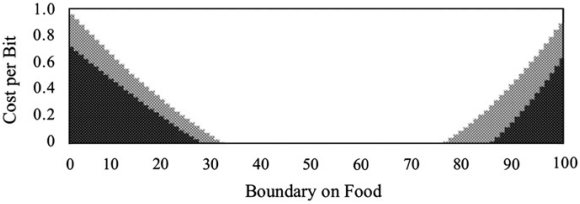
\includegraphics[width=13cm]{Bilder/Single_Resource_Game.png}
  \caption{Genau wahrnehmende Agenten gegen ungenau wahrnehmende}
  \label{fig:srgame}
\end{center}\end{figure}

Die genauere Wahrnehmung gibt es nicht umsonst. Jedes zusätzliche Bit an Information kostet Energie und Zeit. Die genau wahrnehmenden Agenten entscheiden sich erst für ein Territorium, wenn sie genau wissen, wieviel Futter 0..100 darin ist. Die ungenauen Agenten entscheiden aufgrund eines Schwellwerts (boundary) zunächst, ob das Territorium eines mit viel oder wenig Futter ist, und dann für das Territorium mit dem vielen Futter. Die grauen Parameterbereiche bedeuten eine Koexistenz beider Arten. In den schwarzen Bereichen überleben nur die genau wahrnehmenden Agenten, im weißen nur die ungenau wahrnehmenden. Haben die ungenau wahrnehmenden Agenten nur einen halbwegs vernünftigen Schwellwert, dann verdrängen sie die genauen Agenten sogar unabhängig von den Informationskosten.

Ein anderes interessantes Ergebnis, das zeigt, wie wir ticken, wird durch Agenten mit mehr und mehr Kategorien, also nicht nur zweien, erhalten. 
\begin{figure}[!h]\begin{center}
  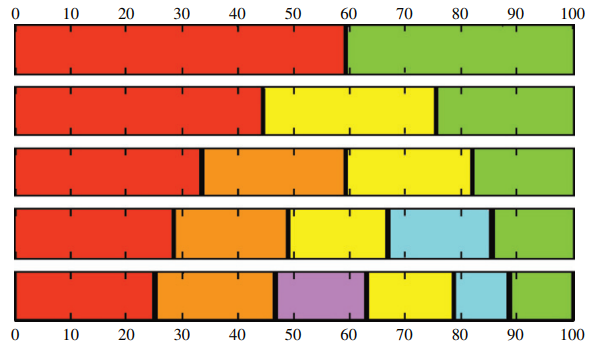
\includegraphics[width=13cm]{Bilder/nCat_Agenten.png}
  \caption{Optimale Postition der Schwellwerte bei verschiedener Anzahl an Kategorien}
  \label{fig:srgame}
\end{center}\end{figure}
Es ist günstig, die Dinge dort genauer zu wissen, wo es etwas zu holen gibt. Wo es nichts zu holen gibt, da haben wir weniger Kategorien. Man könnte es überspitzt auch so sagen: wir haben keine Wörter für Dinge, die es vielleicht geben mag, die uns aber im Hinblick auf unser Überleben nicht interessieren.

\section{Information}
\section{Bedeutung}
\section{Intelligenz}


\end{document}